
\section{Description of the IMMD System}

The IMMD system is composed of 4 identical modules which are to be connected in 2-series and 2-parallel fashion on the DC link. A 2 kW 3-phase GaN based motor drive inverter modules printed circuit board (PCB) and a control and power distribution PCB are designed for the system. The specifications are listed in Table \ref{table:specifications}.


\begin{table}[h]
    \caption{IMMD system specifications}
    \label{table:specifications}
    \centering
    \begin{tabular}{c c c c}
        \toprule
        Parameter & Value & Parameter & Value \\
        \hline
        Total output power & 8 kW & DC link voltage & 540 V \\
        Number of modules & 4 & Motor speed & 600 rpm \\
        Phase induced voltage & 80 Vrms & Line current & 8.5 A \\
        GaN breakdown voltage & 650 V & GaN continuous current & 30 A \\
        \bottomrule
    \end{tabular}
    \vspace{-10pt}
\end{table}

\subsection{GaN based motor drive module}

The picture of the GaN based 3-phase inverter module of the IMMD system is shown in Fig. \ref{fig:invertermodule} excluding the heat sink. The module consists of half-bridge legs with GaN FETs. Each leg has a 5 $\mu F$ metal film capacitor, isolated gate driver circuit dedicated to each GaN and a phase current measurement circuit. In order to overcome the challenge of size reduction due to integration, it is aimed to reduce the size of DC link capacitors and heat sink by utilizing GaN FETs at high switching frequency. The DC link capacitor size is determined according to required capacitance which is calculated based on voltage ripple and required current rating \cite{Ugur2017}, by also taking the effect of interleaving into account. The layout design is based on keeping gate loop and power loop inductances as well as keeping DC link capacitors as close as possible. Ceramic capacitors are also added to the half-bridge layout to reduce the voltage overshoots.

\begin{figure}
\begin{minipage}[b]{.4\linewidth}
\centering
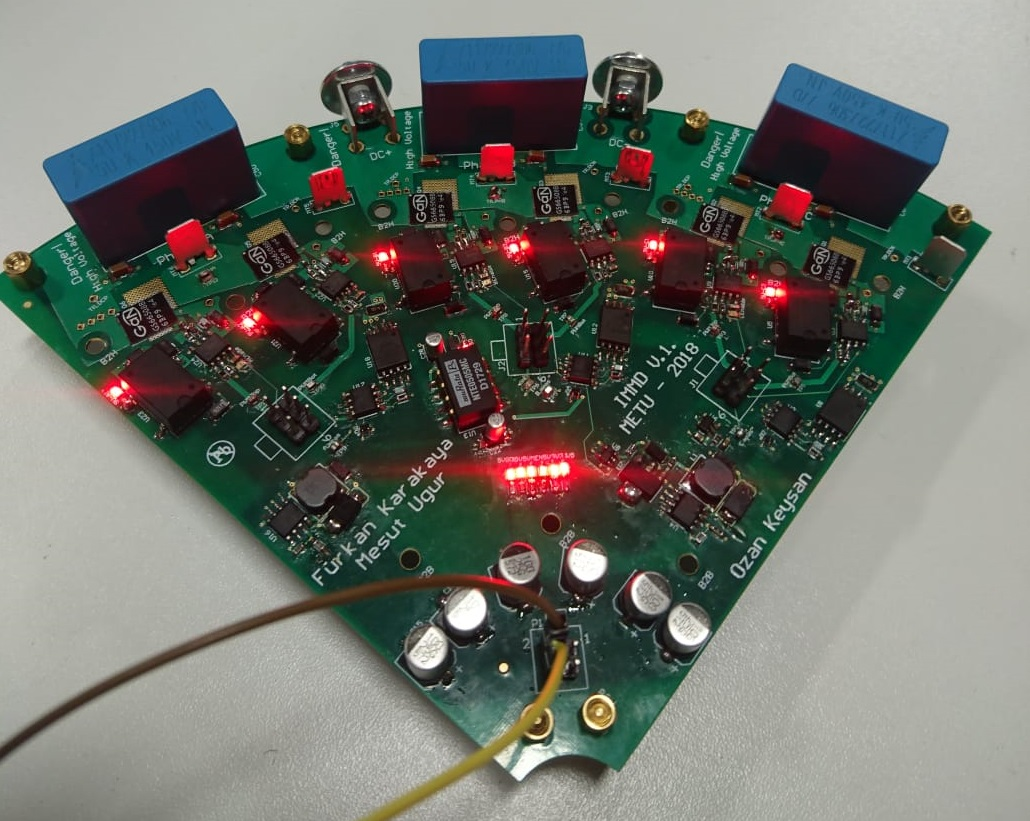
\includegraphics[width=6cm]{figures/invertermodule.jpg}
\caption{GaN based 3-phase inverter module}
\label{fig:invertermodule}
\end{minipage}%
\begin{minipage}[b]{.6\linewidth}
\centering
\subfloat[\label{fig:SeriesModules}Series]{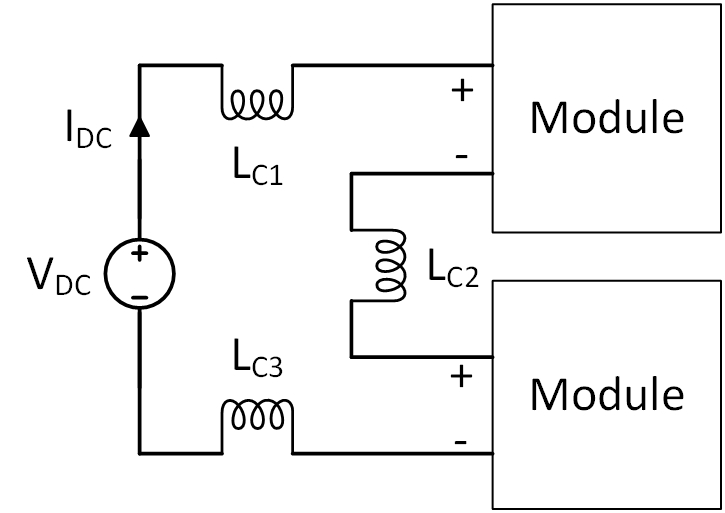
\includegraphics[width=4.5cm]{figures/SeriesModules.jpg}}\quad
\subfloat[\label{fig:ParallelModules}Parallel]{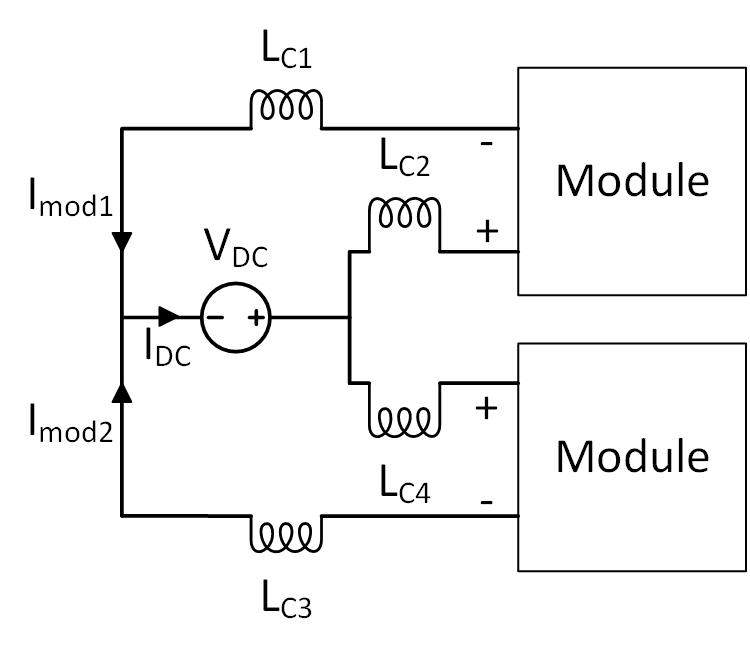
\includegraphics[width=4.5cm]{figures/ParallelModules.jpg}}
\caption{Series and Parallel Connected Modules Configurations}
\label{fig:ModuleConnections}
\end{minipage}
\end{figure}

\subsection{Parasitic inductances}

In physical realization of power electronics circuit, the parasitic inductances of the layout is an important consideration especially for the paths carrying switched current.
For the inverter circuit given in Fig. \ref{fig:invertermodule}, the power loop and commutation loop inductances are identified using Ansys Q3D tool and given in Fig. \ref{fig:SingleModuleInductanceMap}. The power loop is a closed path including half-bridge switches, a DC link capacitor and parasitic inductances which connects them each other . Another closed path is the commutation loop which includes two DC link capacitors and the parasitic inductances between the capacitors. The commutation loop is effective between any two phases of the system whenever a current commutes from one phase to another one. In the following sections, these two loops will be discussed in detail.

\begin{figure}
    \centering
    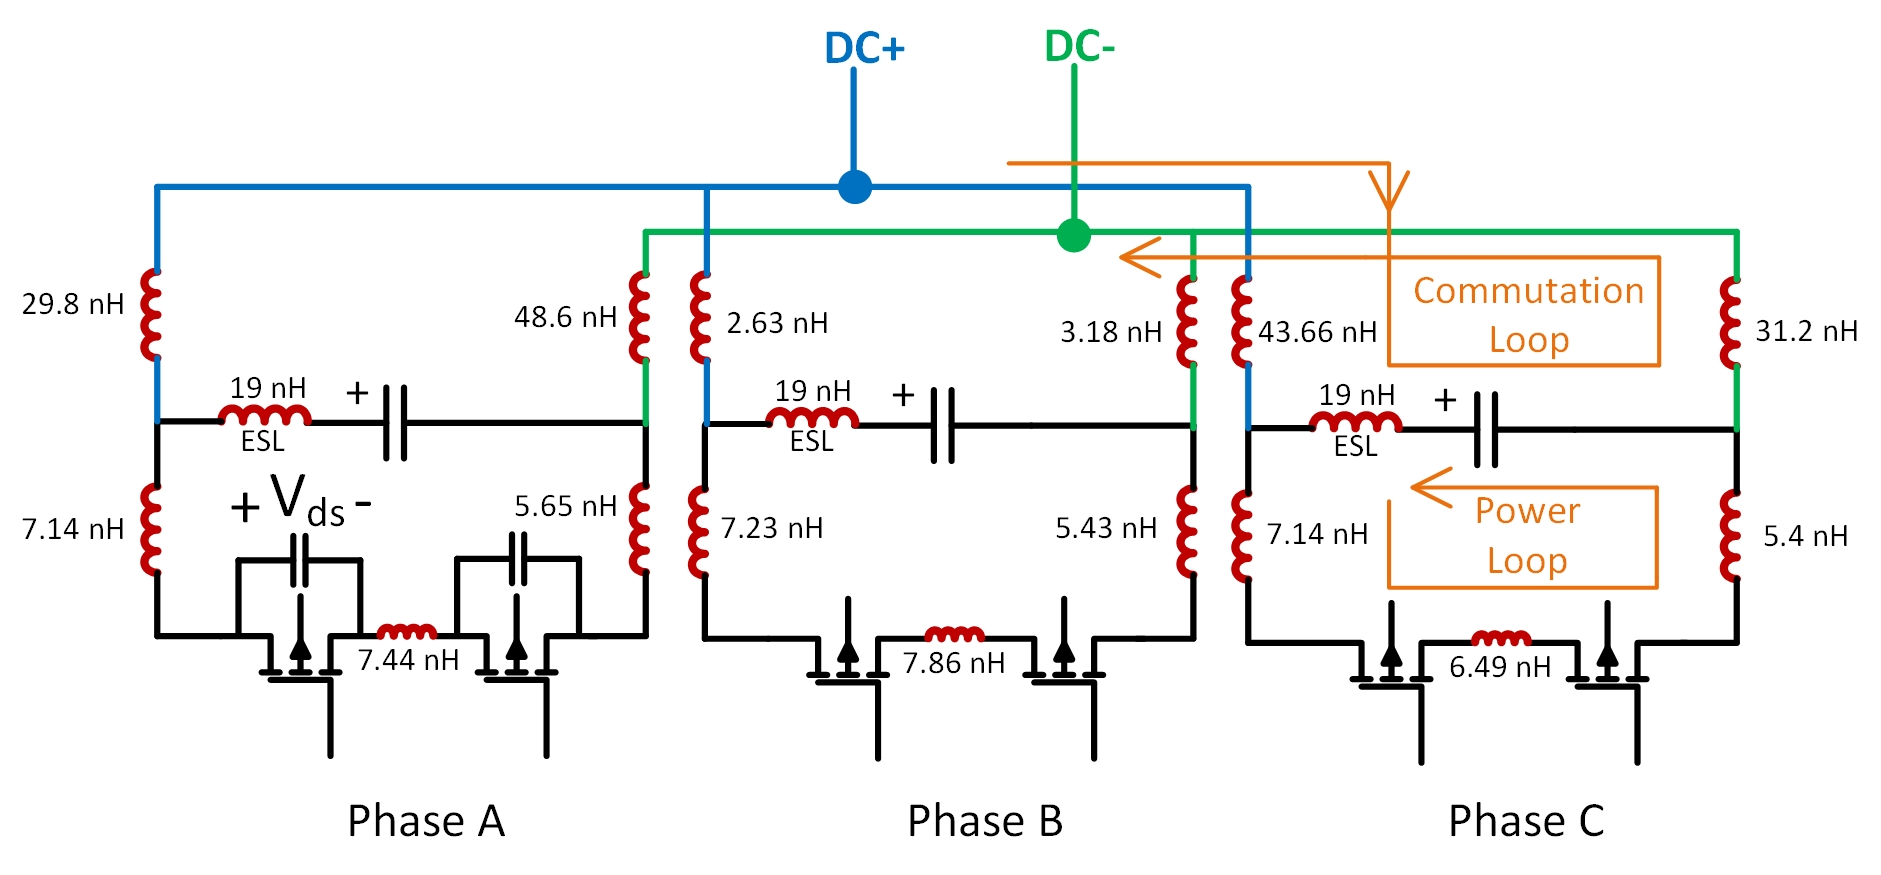
\includegraphics[width=0.8\textwidth]{figures/SingleModuleInductanceMap.jpg}
    \caption{Parasitic Inductance Map of a Single Module}
    \label{fig:SingleModuleInductanceMap}
\end{figure}


%Phase commutation inductances

%Dc bus modelimiz


\subsection{Series and Parallel Connection}

As shown in Fig. \ref{fig:ModuleConnections}, two modules can be connected in series or parallel. The inductances given in Fig. \ref{fig:SeriesModules}, $L_{C1}, L_{C3}$, are total equivalent inductors of connectors and module to supply terminal connections. Similarly, $L_{C2}$ represents the total inductance of connectors and module to module connection. In addition, the equivalent inductors are shown in Fig. \ref{fig:ParallelModules} for parallel connection where $L_{C1} \And L_{C3}$, $L_{C2} \And L_{C4}$  represents the total equivalent inductance from module to supply negative and positive terminals, respectively.


%%Seri ve paralel bağantı nasıl oluyor (figür koyalım)


%%Module connection inductances - notation-figür ve anlatımı

